\documentclass[a4paper, 12pt]{article}
\usepackage[utf8]{inputenc}
\usepackage[T1]{fontenc}
\usepackage{textcomp, color, amsmath, amssymb, tikz, subfig, float, mathrsfs}
\usepackage{xcolor}
\usepackage{amsfonts}
\usepackage{graphicx}
\usepackage{listings}
\usepackage{ragged2e}
\usepackage{amsmath}
\usepackage[export]{adjustbox}
\usepackage[]{esint}
\usepackage{hyperref}
\usepackage[skins,theorems]{tcolorbox}
\tcbset{highlight math style={enhanced,
  colframe=red,colback=white,arc=10pt,boxrule=0.5pt, hbox}}

\definecolor{lightgray}{gray}{0.75}

\newcommand\greybox[1]{%
  \vskip\baselineskip%
  \par\noindent\colorbox{lightgray}{%
    \begin{minipage}{\textwidth}#1\end{minipage}%
  }%
  \vskip\baselineskip%
}
	



\begin{document}



\author{Kristian Tuv}
\title{Studies of phase transitions in magnetic systems}
\maketitle
Link to the code: \url{https://github.com/kristtuv/FYS3150/tree/master/Project4}
\newpage
\tableofcontents
\newpage

Kan også ha aktuelle subseksjoner
\section{Abstract}
We study the Ising model in two dimensions finding the number of Monte Carlo cycles needed to reach a steady state of the system, properties of the system at different temperatures and properties of the system at the critical temperature.
\\
We found that we need 10 000 Monte Carlo cycles to reach a steady state for a 20x20 lattice and the system fluctuates more around the expected energy for higher temperatures.\\
The Ising model can be used to find the critical temperature, but we need more data close the the critical limit than we get from $2 \times 10^6$ Monte Carlo cycles, and we found that at the critical temperature the system experiences a phase transition and transforms from a ferromagnet to a paramagnet.

\section{Introduction}

The aim of this project is to study a widely popular model to simulate phase transitions, the Ising model in two dimensions. At a given critical temperature, this model exhibits a phase transition from a magnetic phase (a system with a finite magnetic moment) to a phase with zero magnetization. We know from Lars Onsager that the critical temperature for a two dimiensional Ising model with the conditions we will set below is $\approx 2.269$\\
In our quest to find the critical temperature we will first test our code aginst analytical results for a 2x2-lattice and then find properties as the steady-state of system starting with a random initial configuration, and the probability of finding a system in a certain state if we start the system at different temperatures. \\

To find the critical termperature for different lattice sizes, we will run the program using parallelization with MPI.

\newpage
\section{Theory and methods}
All the theory in this chapter is gathered from M. Hjort-Jensen, Computational Physics, Lecture Notes Fall 2015, chapter 13\\
\subsection{Mathematical theory}




In our studies of phase transitions at finite temperature for magentic systems we will be using the Ising model. In this model the energy is expressed as 
$$E = -J\sum^{N}_{<kl>}s_{k}s_{l} - \mathscr{B}\sum^{N}_{k}s_{k}$$
with $s = \pm 1$ representing the direction of the spins, N is the total number of spins in the system of particles, J is the coupling constant expressing the strength of the interaction between neighboring spins and $\mathscr{B}$ is an external magnetic field interacting with the magnetic moment set up by the spins. <kl> indicates that we sum over the nearest neighbors of each particle only.\\ In this project we will set $\mathscr{B} = 0$. We will also work with a lattice in two dimentions, which gives and Energy equation for a state i:
$$E_{i} = -J\sum^{N}_{k, l = 1}(s_{k, l}s_{k, l+1} + s_{k, l}s_{k+1, l})$$
This equation sums over all the spins in the lattice, however we encounter a problem when the sum reaches N. We will solve this by having periodic boundary conditions. This means that when we reach the end of the lattice, we will simply jump to the start of the lattice again.\\
We can represent the spins with arrows $\uparrow$ for $s = +1$ and $\downarrow$ for $s = -1$\\
As a demonstration of the metod of summing up the energy we look at a 4x4 lattice: 

\begin{align*}
& \color{black}{\uparrow}\ \color{blue}{\uparrow}\ \color{black}{\uparrow}\ \color{black}{\uparrow} \qquad \color{black}{\uparrow}\ \color{black}{\uparrow}\ \color{blue}{\uparrow}\ \color{black}{\uparrow} \qquad \color{black}{\uparrow}\ \color{black}{\uparrow}\ \color{black}{\uparrow}\ \color{blue}{\uparrow} \\
%
& \color{black}{\uparrow}\ \color{red}{\uparrow}\ \color{blue}{\uparrow}\ \color{black}{\uparrow}\; \; \color{black}{\rightarrow}\; \, \color{black}{\uparrow}\ \color{black}{\uparrow}\ \color{red}{\uparrow}\ \color{blue}{\uparrow}\; \; \color{black}{\rightarrow}\; \, \color{blue}{\uparrow}\ \color{black}{\uparrow}\ \color{black}{\uparrow}\ \color{red}{\uparrow} \\
% 
& \color{black}{\uparrow}\ \color{black}{\uparrow}\ \color{black}{\uparrow}\ \color{black}{\uparrow} \qquad
\color{black}{\uparrow}\ \color{black}{\uparrow}\ \color{black}{\uparrow}\ \color{black}{\uparrow} \qquad \color{black}{\uparrow}\ \color{black}{\uparrow}\ \color{black}{\uparrow}\ \color{black}{\uparrow}\\
%
& \color{black}{\uparrow}\ \color{black}{\uparrow}\ \color{black}{\uparrow}\ \color{black}{\uparrow} \qquad
\color{black}{\uparrow}\ \color{black}{\uparrow}\ \color{black}{\uparrow}\ \color{black}{\uparrow} \qquad \color{black}{\uparrow}\ \color{black}{\uparrow}\ \color{black}{\uparrow}\ \color{black}{\uparrow}\\
\end{align*}
The red arrow is the spin $s_{k,l}$ we are looking at and the blue arrows are the spins $s_{k, l+1}$ and $s_{k+1, l}$ we are multiplying with the red arrow . As we sum up the red arrow eventually reaches the end of the lattice, the blue arrow then jumps to the other side. This is also the case in the vertical direction.\\
\\
The magnetization is defined as:\\
$$\mathscr{M}_{i} = \sum_{j = 1}^{N}s_{j} $$

Where we sum over all spins of a given configuration i.

\subsubsection{Analytic results}
To check the results from our code, we will calculate some values analytically. To do that we need some definitions:\\
\\Boltzmann distribution\footnote{In statistical mechanics and mathematics, a Boltzmann distribution (also called Gibbs distribution[1]) is a probability distribution, probability measure, or frequency distribution of particles in a system over various possible states. Wikipedia: \url{https://en.wikipedia.org/wiki/Boltzmann_distribution}, 15.112016}:\\
$$P_{i}(\beta) = \frac{e^{\beta E_{i}}}{Z}$$ 
with$\beta = 1/kT$, k the Boltzmann constant, $E_{i}$ is the energy of a state i, while Z is the partition function for the canonical ensemble defined as:
$$ Z = \sum^{M}_{i =1} e^{\beta E_{i}} $$

The expectationcalue for a canonical ensemble is defines as:
$$\langle E \rangle = k_{b}T^{2}\left(\frac{\partial lnZ}{\partial T}\right)_{V,N}$$
or using the probability distribution:
$$\langle E \rangle = \sum^{M}_{i = 1}E_{i}P_{i}(\beta) = \frac{1}{Z}\sum^{M}_{i = 1}E_{i}e^{-\beta E_{i}}$$
Where M is the total number of possible microstates in the system.\\
The spesific heat at constant volume:
$$C_{v} = \frac{1}{k_{b}T^{2}}\left(\langle E^{2}\rangle - \langle E \rangle^{2}\right)$$

The expectationvalue of the magnetization:
$$\langle \mathscr{M}\rangle = \sum^{M}_{i}\mathscr{M}_{i}P_{i} = \frac{1}{Z}\sum^{M}_{i}\mathscr{M}_{i}e^{-\beta E_{i}}$$
In a square lattice, this value will always be zero because for every magnetization, we can always find an equal number of states with the same magnetization but with the opposite sign. Because of this we will instead look at the expectation value of the absolute value:
$$\langle |\mathscr{M}|\rangle = \sum^{M}_{i}|\mathscr{M}|_{i}P_{i} = \frac{1}{Z}\sum^{M}_{i}|\mathscr{M}|_{i}e^{-\beta E_{i}}$$

The susceptibility\footnote{The susceptibility indicates whether a material is attracted into or repelled out of a magnetic field, Wikipedia: \url{https://en.wikipedia.org/wiki/Magnetic_susceptibility} , 15.11.2016}:
$$\chi = \frac{1}{k_{b}T}\left(\langle\mathscr{M}^{2}\rangle - \langle |\mathscr{M}| \rangle ^{2}\right)$$
%These results are important because when we increase the size of the lattice, we are still asuming that the direction of a spin only %depends on the 4 closest spins. This means that when we go through the lattice calculating the energy, every calculation can only %take the values -8J, 

We take a look at all the possible microstates for the 2 dimensional Ising-model with 2 x 2 spins and periodic boundary conditions:\\
\\
\begin{tabular}{| r | r | r | r |}
\hline

Number spins up & Degeneracy & Energy & Magnetization\\
\hline
4 & 1 & -8J & 4\\
3 & 4 & 0 & 2\\
2 & 4 & 0 & 0\\
2 & 2 & 8J & 0\\
1 & 4 & 0 & -2\\
0 & 1 & -8J & -4\\
\hline
\end{tabular}\\

To make our calculations simpler, we will set the Boltzman constant $k_{b} = 1$ and the coupling constant $J = 1$. This gives the temperature $T$ units energy. For $T = 1$ and using the results from the tabular in our equations we get:
$$\langle E \rangle = \frac{-8 e^{8} + 8e^{8}}{e^{8} + e^{-8} + 6} \approx -7.983928$$\\
$$Cv = \frac{64(6e^{8} + 6e^{-8} + 4)}{(e^{8} + e^{-8} + 6)^{2}} \approx 0.128329$$\\
$$\langle |M| \rangle = \frac{4(e^{8} + 2)}{e^{8} + e^{-8} + 6} \approx 3.994643$$\\
$$\chi = \frac{16(3e^{8} + e^{-8} + 3}{(e^{8} + e^{-8} +6)^2} \approx 0.016043$$\\

\subsubsection{Phase Transitions}
Through finite size scale relations\footnote{Computational physics, project 4, M. Hjort-Jensen, \url{https://github.com/CompPhysics/ComputationalPhysics/blob/gh-pages/doc/Projects/2016/Project4/pdf/Project4.pdf}} it is possible to relate the behavior at finite size lattices with the results for  an infinitely large lattice. The critical temperature scales then as 
$$T_{C}(L) - T_{C}(L = \infty) = aL^{-1/\nu}$$
We will try to extract the critical temperature of the system by using different sized lattices and subtracting the equations.
\begin{align*}
T_{C}(L_{i}) - T_{C}(L = \infty) - (T_{C}(L_{j}) - T_{C}(L = \infty)) &= aL_{i}^{-1/\nu} - aL_{j}^{-1/\nu} \\
\rightarrow a &=  \frac{T_{C}(L_{i}) - T_{C}(L_{j})}{L_{i}^{-1/\nu} - aL_{j}^{-1/\nu}}
\end{align*}
When we find an estimate for a, we can use:
$$ T_{C}(L = \infty) = - aL_{i}^{-1/\nu} + T_{C}(L_{i})$$
\subsection{Algorithms}
\subsubsection{The Metropolis Algorithm and the two diminsional Ising model}
We will be using the Metropolis algorithm for solving the Ising model. In this algorithm new configurations are generated from a previous configuration using a transition probability which depends on the energy difference between the initial and final states. In our case we are using the Boltzman distribution as our probability function:
$$P_{i} = \frac{e^{-\beta E_{i}}}{Z}$$
With $E_{i}$ the energy for a state i, $\beta = 1/kT$ and Z a normalization constant which defines the partition function in the canonical ensemble
$$Z = \sum_{i} e^{-\beta E_{i}}$$
Z is difficult to compute, since we need all states. In a calcualtion of the Ising model in two dimensions, the number of configurations is given by $2^N$ with $N = L \times L$ the number of spins for a lattice of length L. However we will only concider the ratio between probabilites in the Metropolis Algorithm:
$$w = \frac{P_{t}}{P_{b}} = \frac{\frac{e^{-\beta E_{t}}}{Z}}{\frac{e^{-\beta E_{b}}}{Z}} = e^{-\beta E_{t}} e^{\beta E_{b}} = e^{-\beta (E_{t} - E_{b})} = e^{-\beta \Delta E}$$
Where $E_{b}$ is the energy in our initial state and $E_{t}$ is a trial energy we get from flipping one spin in our state.
Before describing the algorithm, we need to take a quick look at our energy calculation. If we position ourselves on a random spin in our lattice, the spin can only be affected be the 4 closest spins. Because we are limiting ourselves to flipping one spin at a time, there is only a limited number of values for the energy changes:
\begin{minipage}{0.45\textwidth}
\begin{align*}
&\uparrow\\
E = -4J  \qquad \qquad \uparrow &\uparrow\ \uparrow \qquad \qquad \qquad\Longrightarrow\\
&\uparrow\\
\end{align*}
\end{minipage}
\begin{minipage}{0.45\textwidth}
\begin{align*}
&\uparrow\\
E = 4J \qquad \qquad  \uparrow &\downarrow\ \uparrow \qquad \\
&\uparrow\\
\end{align*}
\end{minipage}\\
\\
With $\Delta E = 8J$\\
\\
\\
\begin{minipage}{0.45\textwidth}
\begin{align*}
&\uparrow\\
E = -2J  \qquad \qquad \uparrow &\uparrow\ \uparrow \qquad \qquad \qquad\Longrightarrow\\
&\uparrow\\
\end{align*}
\end{minipage}
\begin{minipage}{0.45\textwidth}
\begin{align*}
&\uparrow\\
E = 2J \qquad \qquad  \uparrow &\downarrow\ \uparrow \qquad \\
&\uparrow\\
\end{align*}
\end{minipage}\\
\\
With $\Delta E = 4J$\\
\\
\\
\begin{minipage}{0.45\textwidth}
\begin{align*}
&\uparrow\\
E = 0 \qquad \qquad \uparrow &\uparrow\ \uparrow \qquad \qquad \qquad\Longrightarrow\\
&\uparrow\\
\end{align*}
\end{minipage}
\begin{minipage}{0.45\textwidth}
\begin{align*}
&\uparrow\\
E = 0\qquad \qquad  \uparrow &\downarrow\ \uparrow \qquad \\
&\uparrow\\
\end{align*}
\end{minipage}\\
\\
With $\Delta E = 0$\\
\\
\\
\begin{minipage}{0.45\textwidth}
\begin{align*}
&\uparrow\\
E = 2J  \qquad \qquad \uparrow &\uparrow\ \uparrow \qquad \qquad \qquad\Longrightarrow\\
&\uparrow\\
\end{align*}
\end{minipage}
\begin{minipage}{0.45\textwidth}
\begin{align*}
&\uparrow\\
E = -2J \qquad \qquad  \uparrow &\downarrow\ \uparrow \qquad \\
&\uparrow\\
\end{align*}
\end{minipage}\\
\\
With $\Delta E = -4J$\\
\\
\\
\begin{minipage}{0.45\textwidth}
\begin{align*}
&\uparrow\\
E = 4J  \qquad \qquad \uparrow &\uparrow\ \uparrow \qquad \qquad \qquad\Longrightarrow\\
&\uparrow\\
\end{align*}
\end{minipage}
\begin{minipage}{0.45\textwidth}
\begin{align*}
&\uparrow\\
E = -4J \qquad \qquad  \uparrow &\downarrow\ \uparrow \qquad \\
&\uparrow\\
\end{align*}
\end{minipage}\\
\\
With $\Delta E = -8J$\\
\\
\\
As we can see there is only five possible values for the energy difference. Which means we can calculate all the probabilities $$w = e^{-\beta \Delta E}$$ in advance and save a ton of computning power because we do not have to evaluate the exponential at each Monte Carlo sampling.

\greybox{
1. Establish an initial state using a random number generator that produces numbers 1 or -1. The state has the initial energy $E_{b}$. Positioning yourself at a random configuration in the lattice.\\
2. Change the initial configuration by flipping on spin only. Compute the energy of this trial state $E_{t}$\\
3. Calculate $\Delta E = E_{t} - E_{b}$. The number of values $\Delta E$ is limited to the five values discussed above.\\
4. If $\Delta E \leq 0 $ we accept the new configuration, meaning that the energy is lowered and we are moving towards the energy minimum at a given temperature. Go to step 7. *\\
5. If $\Delta E > 0$, calculate $w = e^{-\beta \Delta E}$\\
6. Compare w with a random number r. If
$$r \leq w,$$
then acccept the new configuration, else we keep the old configuration.\\
7. Update various expectations values.\\
8. Repeat steps 2-7 in order to obtain a sufficently good representation of states.\\
9. Each sweep through the lattice is one Monte Carlo cycle. At the end you should divide the various expecttation values with the total number of cycles.\\}
* In the 2-dim Ising Model with J=1 and k=1, this step can be skipped because the values we can get for $\Delta E$ is -8J, -4J, 0, 4J and 8J, . Our random number r is produced from a uniform distribution between 0 and 1 and $e^{-(-8)}, e^{-(-4)}, e^{-(0)}$ is always greater or equal to one, which means step 6 includes step 4.\\


\section{Results}

The algorithm was tested for a 2x2-lattice with the calculated expectationvalues given in expectation value per spin. In other words, the expectation values we found in the mathematical theory section has all been devided by four.\\
The initial lattice was set to the ground state with all spins pointing up to make the expectation value as close to the analytical as possible.\\
The Mersenne Twister 19937 generator (64 bit) was used as a random number generator, which has a period of $\approx 4.3×10^6001$ \footnote{\url{https://en.wikipedia.org/wiki/Pseudorandom_number_generator}, 16.11.2016}\\
\\
\begin{tabular}{| r | r | r | r | r |}
\hline
&- &Analytical &Nummerical: $MCc=10^{4}$ &Nummerical: $MCc=10^{6}$\\
\hline
&$\langle E\rangle$ &-1.995982 &-1.9956000 &-1.9959080\\
&$C_{v}$ &0.032082 &0.035122560 &0.032669022\\
&$\langle |M|\rangle$ &0.998661 &0.99840000 &0.99863000\\
&$\chi$ & 0.004011 &0.0051897600 &0.0041204924\\
\hline
\end{tabular}
\\
As we can see from the tabular, all the expectationvalues start getting pretty accurate already at $10^4$ Monte Carlo cycles.\\ Normally we will start the simulation in a random state and not in the ground state. Because of this we will normally want to exclude a portion of the cycles in the beginning, so generally $10^4$ cycles might be a bit risky if we want to get a good result.\\
\\
To find out how many simulations we actually need to reach the steady state, we have plotet the various expectations values as a function of Monte Carlo cycles\\
The program was run for $10, 10^2, 10^3, 10^4, 10^5, 10^6$ Monte Carlo cycles.
\begin{figure}[H]
\centering
\subfloat[Starting simulation from ground state]{\includegraphics[width=0.55\textwidth]{/Users/Tuv/Documents/Programming/FYS3150/Project4/build-Project4-Desktop_Qt_5_7_0_clang_64bit-Profile/Savefiles/Eground.png}}
\subfloat[Starting simulation from random state]{\includegraphics[width=0.55\textwidth]{/Users/Tuv/Documents/Programming/FYS3150/Project4/build-Project4-Desktop_Qt_5_7_0_clang_64bit-Profile/Savefiles/Erandom.png}}
\caption{$\langle E\rangle$.}
\end{figure}
%%%
\begin{figure}[H]
\centering
\subfloat[Starting simulation from ground state]{\includegraphics[width=0.55\textwidth]{/Users/Tuv/Documents/Programming/FYS3150/Project4/build-Project4-Desktop_Qt_5_7_0_clang_64bit-Profile/Savefiles/Cvground.png}}
\subfloat[Starting simulation from random state]{\includegraphics[width=0.55\textwidth]{/Users/Tuv/Documents/Programming/FYS3150/Project4/build-Project4-Desktop_Qt_5_7_0_clang_64bit-Profile/Savefiles/Cvrandom.png}}
\caption{$C_{V}$.}
\end{figure}
%%%
\begin{figure}[H]
\centering
\subfloat[Starting simulation from ground state]{\includegraphics[width=0.55\textwidth]{/Users/Tuv/Documents/Programming/FYS3150/Project4/build-Project4-Desktop_Qt_5_7_0_clang_64bit-Profile/Savefiles/Mground.png}}
\subfloat[Starting simulation from random state]{\includegraphics[width=0.55\textwidth]{/Users/Tuv/Documents/Programming/FYS3150/Project4/build-Project4-Desktop_Qt_5_7_0_clang_64bit-Profile/Savefiles/Mrandom.png}}
\caption{$\langle |M| \rangle$.}
\end{figure}
\begin{figure}[H]
\centering
\subfloat[Starting simulation from ground state]{\includegraphics[width=0.6\textwidth]{/Users/Tuv/Documents/Programming/FYS3150/Project4/build-Project4-Desktop_Qt_5_7_0_clang_64bit-Profile/Savefiles/Xground.png}}
\subfloat[Starting simulation from random state]{\includegraphics[width=0.6\textwidth]{/Users/Tuv/Documents/Programming/FYS3150/Project4/build-Project4-Desktop_Qt_5_7_0_clang_64bit-Profile/Savefiles/Xrandom.png}}
\caption{$\chi$.}
\end{figure}
As we can see, the steady state is in fact more or less reached at 10 000 Monte Carlo cycles. To make the expectation values as accurate as possible we need to start our expectation values-sampling after the 10 000th cycle. However, to be on the safe side I have removed the first 10 percent of the total number of cycles to ensure steady state in the continued part of the project.\\
Looking at the expectation values of $T=2.4$ when starting the simulation in the ground state, in the lowest energy state, it does not stay at more or less the same value, as it does with $T=1.0$. To find out why we take a look at the number of accepted configurations as a function of Monte Carlo cycles.


\begin{figure}[H]
\centering
\subfloat[Simulate from ground state. Logarithm on axis]{\includegraphics[width=0.6\textwidth]{/Users/Tuv/Documents/Programming/FYS3150/Project4/build-Project4-Desktop_Qt_5_7_0_clang_64bit-Profile/Savefiles/AcceptedT1ground.png}}
\subfloat[Simulate from random state. Logarithm on axis]{\includegraphics[width=0.6\textwidth]{/Users/Tuv/Documents/Programming/FYS3150/Project4/build-Project4-Desktop_Qt_5_7_0_clang_64bit-Profile/Savefiles/AcceptedT1random.png}}\\
\subfloat[Simulate from ground state. Logarithm on axis]{\includegraphics[width=0.6\textwidth]{/Users/Tuv/Documents/Programming/FYS3150/Project4/build-Project4-Desktop_Qt_5_7_0_clang_64bit-Profile/Savefiles/AcceptedT2ground.png}}
\subfloat[Simulate from random state. Logarithm on axis]{\includegraphics[width=0.6\textwidth]{/Users/Tuv/Documents/Programming/FYS3150/Project4/build-Project4-Desktop_Qt_5_7_0_clang_64bit-Profile/Savefiles/AcceptedT2random.png}}
\caption{Plots of the accepted number of configurations as a function of Monte Carlo cycles. The logarithm is used on both axis to fit all the points in one plot}
\end{figure}
As we can see from Figure 5, the number of accepted configrations as a function of Monte Carlo cycles is a linear function. This is an expected result because we are using a uniform distribution when comparing with our probability $w = e^{-\beta \Delta E}$ and the number of times we get an accepted configuration should increase about a factor of 10 if we increase the number of Monte Carlo cycles with a factor of 10.\\
We can also se that we get a lot more accepted configurations with a higher temperature, this is because increasing the temperature also increases the probability we are comparing our random number with and hence increases the chance of getting a new configuration. We can see this from the tabular below.\\
\\
\begin{tabular}{|r|r|r|}
\hline
T = 1.0  &deltaE = -8 	&w= 2980.957 \\
T = 1.0  &deltaE = -4  	&w= 54.59815 \\
T = 1.0  &deltaE =  0 	&w= 1.000000 \\
T = 1.0  &deltaE =  4 	&w= 0.018316 \\
T = 1.0  &deltaE =  8 	&w= 0.000335 \\
\hline
T = 2.4  &deltaE = -8  	&w= 28.03162 \\
T = 2.4  &deltaE = -4  	&w= 5.294490 \\
T = 2.4  &deltaE =  0 	&w= 1.000000 \\
T = 2.4  &deltaE =  4 	&w= 0.188876 \\
T = 2.4  &deltaE =  8 	&w= 0.035674\\
\hline
\end{tabular}
\\
\\
We now know that the chance of getting a new configuration when the temperature is higher is a lot greater than for small temperatures. This emplies that if we plot the probability of E, the graph of $T=2.4$ should be a lot wider than that of $T = 1.0$


\begin{figure}[H]
\centering
\subfloat[T=1.0]{\includegraphics[width=0.55\textwidth]{/Users/Tuv/Documents/Programming/FYS3150/Project4/build-Project4-Desktop_Qt_5_7_0_clang_64bit-Profile/Savefiles/20x20latticeT1.png}}
\subfloat[T=2.4]{\includegraphics[width=0.55\textwidth]{/Users/Tuv/Documents/Programming/FYS3150/Project4/build-Project4-Desktop_Qt_5_7_0_clang_64bit-Profile/Savefiles/20x20latticeT2.png}}
\caption{The probability of finding our system in a certain energy state.}
\end{figure}
We are now looking at the number of times the entire system is found in a certain energy. From our program we calculated $\langle E(T=1.0) \rangle = -1.9971921$ and $\langle E(T=2.4) \rangle = -1.2318673$ for the energy per spin. We now want to total energy of a state, so we multiply with the size of the lattize $20\times 20$ and get $$\langle E(T=1.0) \rangle = -798.87684$$ and $$\langle E(T=2.4) \rangle = -492.74692$$ \\
Our program also calcualtes $C_{v}$. To find $\sigma _{E}$ for the entire system we need to multiply $C_{v}$ by $T^2$ and $20 \times 20$ and take the square root. We get $$\sigma_{E}(T=1.0) = \sqrt{0.0056956373 \times 1.0^2 \times 400} = 1.50938892271$$ and $$\sigma_{E}(T=2.4) = \sqrt{1.4104501\times 2.4^2 \times 400} = 57.0059385538$$.\\
In our plot for $T=2.4$ the standard deviation should contain about 2/3 of our values, which look about right.\\
For $T = 1.0$ we do not have a normal distribution, but the standard deviation is also very small and close to all the values are centered around the ground state, hence our calculations are correct.\\

\paragraph{Finding the critical temperature}
The program ran using parallization with MPI for $2 \times 10^6$ Monte Carlo cycles, with the first 10 percent removed to ensure steady state.\\
Because we already knew the critical temperature, we ran the temperature interval [2.0, 2.22] with a temperature step of 0.02. For the interval [2.22, 2.32] we ran with a step size of 0.005.
\begin{figure}[H]
\centering
\subfloat[]{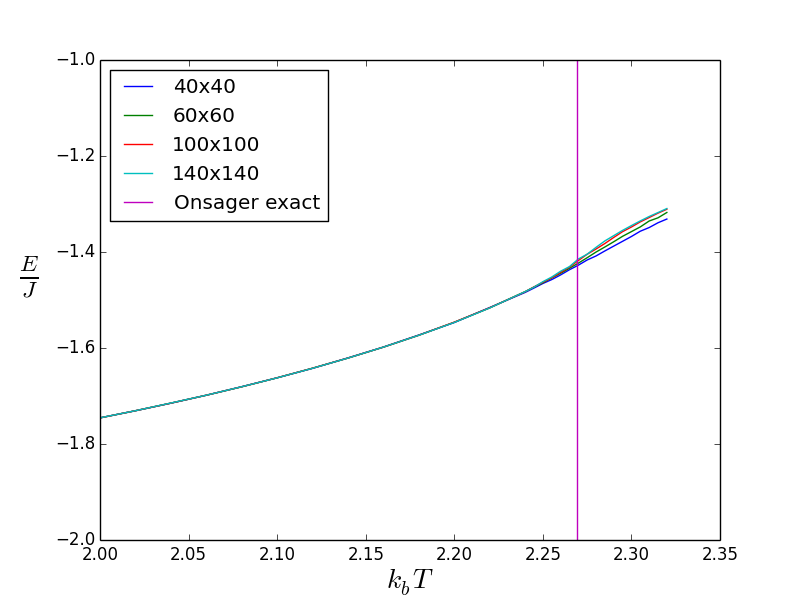
\includegraphics[width=0.55\textwidth]{//Users/Tuv/Documents/Programming/FYS3150/Project4/MPIProject4/E.png}}
\subfloat[Starting simulation from ground state]{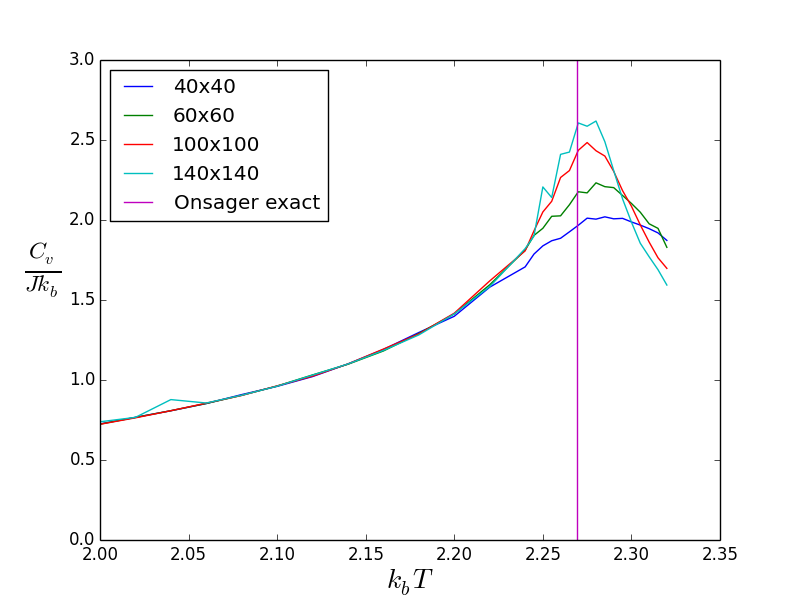
\includegraphics[width=0.55\textwidth]{//Users/Tuv/Documents/Programming/FYS3150/Project4/MPIProject4/Cv.png}}\\
\subfloat[]{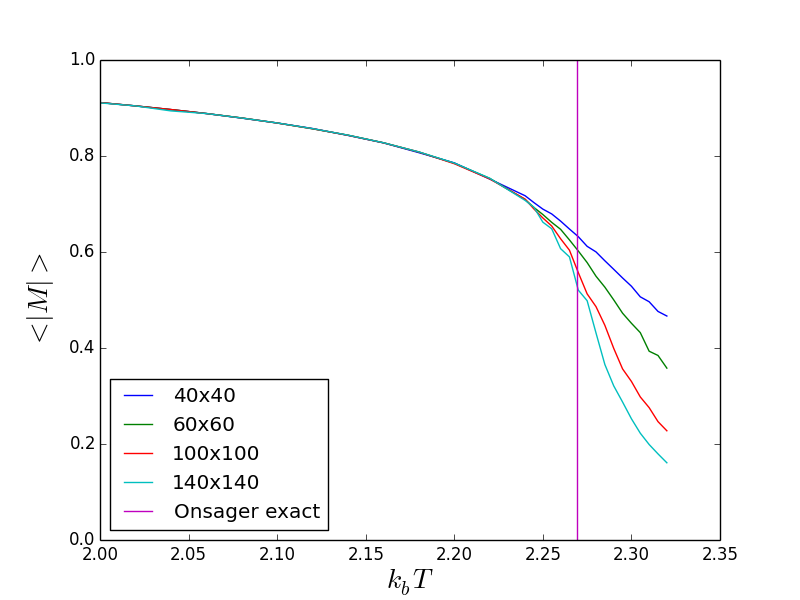
\includegraphics[width=0.55\textwidth]{//Users/Tuv/Documents/Programming/FYS3150/Project4/MPIProject4/M.png}}
\subfloat[]{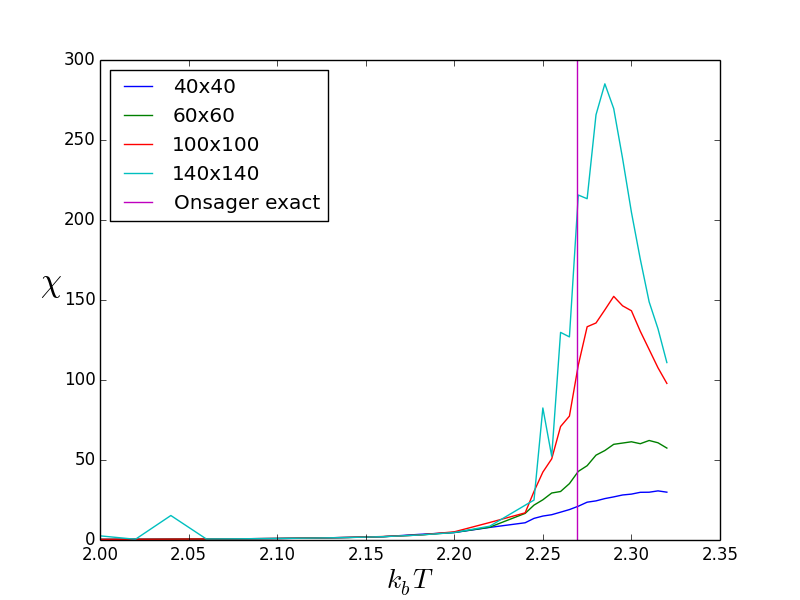
\includegraphics[width=0.55\textwidth]{//Users/Tuv/Documents/Programming/FYS3150/Project4/MPIProject4/Chi.png}}
\caption{Expectationvalues as a function of temperature close to the critical temperature. The purple line is the Lars Onsager exact result for $T_{C}$}
\end{figure}

If we take look at $\langle |M|\rangle$ we see that if we are moving from higher to lower temperature, at the critical temperature the system experiences a spontanious magnetication. This is because at the critical temperature the system goes through a phase transformation. The phase at low temperatures is called a ferromagnetic phase while above $T_{C}$ it is called the paramagnetic phase\footnote{M. Hjort-Jensen, Computational Physics, Fall 2015, Chapter 13, p. 443}. We can see this in the plot. A ferromagnet is a permanent magnet\footnote{\url{https://en.wikipedia.org/wiki/Ferromagnetism}, 16.11.2016} and below $T_{C}$ we always have magnetization. At $T_{C}$ the magnetization drops toward zero and we get a parramagnet\footnote{\url{https://en.wikipedia.org/wiki/Paramagnetism}, 16.11. 2016} where we need an external magnetic field for attraction. In the plot of $Chi$ we can see that the susceptibility rises and the systems ability to be attracted or repelled by a magnet field rises, as we would expect from a paramagnet.\\
From the plots of  $Cv$ we see that tha curves diverge at $T_{C}$. Because the system experiences a phase transition, the system becomes unstable and hence unphysical. In the real world the system would jump from one side of the critical temperature to the other through the phase transition.\\
\\
By looking at the data, we found the following critical temperatures for the different lattice sizes:\\
\\
\begin{tabular}{|r|r|}
\hline
L &$T_{C}$ \\
\hline
40 &2.285\\
60 & 2.280\\
100 & 2.275\\
140 & 2.275\\
\hline
\end{tabular}\\
\\
By using the result:
$$a =  \frac{T_{C}(L_{i}) - T_{C}(L_{j})}{L_{i}^{-1/\nu} - aL_{j}^{-1/\nu}}$$

We compared these lattices to find different estimates for a, an took the average of them:\\
40-60, 40-100, 40-140, 60-100, 60-140 and 100-140\\

The average gave: $a = 0.5169$\\

Then we calculated:\\
$$ T_{C}(L = \infty) = - aL_{i}^{-1/\nu} + T_{C}(L_{i})$$

Which gave the result:\\
$T_{C}(L = \infty ) = 2.2713$\\
\\

This is pretty close to the exact result $T_{C} = 2.269$ but a bit worse than hoped. From the graphs we can see that in the simulation of the interval closest to $T_{C}$ the curve is oscillation a lot. Becase my temperature step is so small, the amount of Monte Carlo cycles should probably have been increased by several factors to get a more accurate result, but to do that we would need a more powerful computer.
\section{Conclusion}
From our study we found that at least for a $20 \times 20$ lattice 10 000 Monte Carlo cycles are enough to reach the steady state of the system. Also the accepted configurations increases for increased T because the comparing probability also increases and the probability of a new state being accepted is much greater than for very small temperatures. This leads to the system not staying in the lowest possible energy state, but fluctuates around a higher temperature.\\
The most important result of the project was finding the critical temperature and the implications of this temperature.\\
We learned that we can find the critical temperature of a system by comparing critical temperatures for different sized lattices, however we need a sufficiently high number of Monte Carlo cycles. When we are dealing with random numbers, the more data we are able to produce, the better the results. Also we only used the Ising model to study our system and, even though it is popular, we did not use any data for comparing the algorithm  with another. For all we know the Ising model might not be the algorithm of choice to get the very best results when studying critical temperatures. \\ We also found that when the system reaches the critical temperature, a phase transition occurs, and the system changes from a ferromagnet to a paramagnet.

\end{document}
